\chapter[Special Surveys]{Special Surveys}
\def\chpname{specialsurveys}\label{chp:\chpname}

Chapter editors:
\credit{dnidever},
\credit{knutago}.

% Confirmed leads for LMC/SMC: Knut Olsen, David Nidever

% Confirmed leads for special surveys:

% --------------------------------------------------------------------

\section{Introduction}
\label{sec:specials:intro}

% Introduce, with a very broad brush, this chapter's science projects,
% and why it makes sense for them to be considered together.

The four main LSST science themes, as defined by the Science Book,
drive the design of LSST's main Wide-Fast-Deep survey.  However, it
has always been recognized that many important scientific projects,
including some that are highly relevant to LSST's main science themes,
are not well served by the areal coverage and/or cadence constraints
placed on the WFD survey.  To this end, the LSST Project set aside a
nominal 10\% of the observing time to serve what are collectively
called ``special surveys''.

Projects that
will certainly make use of this 10\% time (that is not dedicated to the WFD
survey) include the Deep Drilling fields and the Galactic Plane surveys, as well as any survey wishing to
observe at declinations below $-60^\circ$, such as the Magellanic
Clouds.  These special programs heavily oversubscribe the nominal 10\%
of time assigned to them.  It is of thus critical importance for these
programs to define compelling science cases, clearly justify their
observing requirements, and derive metrics to quantify the performance
of a given schedule for the program.
% An extra degree of freedom that these special surveys

A minimal set of 4--5 ``extragalactic'' Deep Drilling Fields have been
included in the `OpSim` runs to date (\autoref{chp:cadexp}), and have
been evaluated in various science sections throughout this paper.
Here, we explore some other proposals for Deep Drilling Fields, and
make some suggestions for \OpSim runs based on them. As well as these
DDF's, we also describe a special survey designed to serve scientific
goals related to the Magellanic Clouds, and \ldots.  Descriptions of
further proposed special surveys are welcome here.

% Add sections below, one science investigation per section, one
% section per file.
% --------------------------------------------------------------------

% ====================================================================
%+
% NAME:
%    magcloudsurvey.tex
%
% CHAPTER:
%    specialsurveys.tex
%
% ELEVATOR PITCH:
%
% AUTHORS:
%    David Nidever (@dnidever)
%    Knut Olsen (@knutago)
%-
% ====================================================================

\section{The Magellanic Clouds Special Survey}
\def\secname{mc}\label{sec:\secname}

\credit{dnidever},
\credit{knutago}.

An LSST survey that did not include coverage of the Magellanic Clouds
and their periphery would be tragically incomplete.  LSST has a unique
role to play in surveys of the Clouds.  First, its large $A\Omega$
will allow us to probe the thousands of square degrees that comprise
the extended periphery of the Magellanic Clouds with unprecedented
completeness and depth, allowing us to detect and map their extended
disks, stellar halos, and debris from interactions that we already
have strong evidence must exist (REFS).  Second, the ability of LSST
to map the entire main bodies in only a few pointings will allow us to
identify and classify their extensive variable source populations with
unprecedented time and areal coverage, discovering, for example,
extragalactic planets, rare variables and transients, and light echoes
from explosive events that occurred thousands of years ago (REFS).
Finally, the large number of observing opportunities that the LSST
10-year survey will provide will enable us to produce a static imaging
mosaic of the main bodies of the Clouds with extraordinary image
quality, an invaluable legacy product of LSST.

% --------------------------------------------------------------------

\subsection{A Proposed Magellanic Clouds Mini-survey}
\label{sec:\secname:proposal}

We propose two distinct mini-surveys to meet the goals of LSST
Magellanic Clouds science:
\begin{itemize}
\item A mini-survey covering the 2700$\deg^2$ with $\delta < -60$ to
the standard LSST single-exposure depth and to stacked depths of XXX,
with cadence sufficient to detect and measure light curves of RR Lyrae
stars.
\item A mini-survey covering $\sim$250$\deg^2$ of the main bodies of
the Clouds with cadence sufficient to detect exoplanet transits and
other variable objects; a subset of these images should be taken with
seeing of $0.5\arcsec$, with stacked depth reaching the confusion
limits in the Clouds.
\end{itemize}

Figure X shows a rough map of the proposed mini-surveys.
% Need the figure and caption


% --------------------------------------------------------------------

\subsection{Mini-survey Impact on the Magellanic Cloud Science Projects}
\label{sec:\secname:revisit}

\new{Here we revisit the metric analysis of the Magellanic  Clouds'
science cases (\autoref{chp:MCs}), and make some predictions about how
they are likely to improve given  the above proposal.}


% --------------------------------------------------------------------

\subsection{Discussion}
\label{sec:\secname:discussion}


% ====================================================================
%
% \subsection{Conclusions}
%
% Here we answer the ten questions posed in
% \autoref{sec:intro:evaluation:caseConclusions}:
%
% \begin{description}
%
% \item[Q1:] {\it Does the science case place any constraints on the
% tradeoff between the sky coverage and coadded depth? For example, should
% the sky coverage be maximized (to $\sim$30,000 deg$^2$, as e.g., in
% Pan-STARRS) or the number of detected galaxies (the current baseline but
% with 18,000 deg$^2$)?}
%
% \item[A1:] ...
%
% \item[Q2:] {\it Does the science case place any constraints on the
% tradeoff between uniformity of sampling and frequency of  sampling? For
% example, a rolling cadence can provide enhanced sample rates over a part
% of the survey or the entire survey for a designated time at the cost of
% reduced sample rate the rest of the time (while maintaining the nominal
% total visit counts).}
%
% \item[A2:] ...
%
% \item[Q3:] {\it Does the science case place any constraints on the
% tradeoff between the single-visit depth and the number of visits
% (especially in the $u$-band where longer exposures would minimize the
% impact of the readout noise)?}
%
% \item[A3:] ...
%
% \item[Q4:] {\it Does the science case place any constraints on the
% Galactic plane coverage (spatial coverage, temporal sampling, visits per
% band)?}
%
% \item[A4:] ...
%
% \item[Q5:] {\it Does the science case place any constraints on the
% fraction of observing time allocated to each band?}
%
% \item[A5:] ...
%
% \item[Q6:] {\it Does the science case place any constraints on the
% cadence for deep drilling fields?}
%
% \item[A6:] ...
%
% \item[Q7:] {\it Assuming two visits per night, would the science case
% benefit if they are obtained in the same band or not?}
%
% \item[A7:] ...
%
% \item[Q8:] {\it Will the case science benefit from a special cadence
% prescription during commissioning or early in the survey, such as:
% acquiring a full 10-year count of visits for a small area (either in all
% the bands or in a  selected set); a greatly enhanced cadence for a small
% area?}
%
% \item[A8:] ...
%
% \item[Q9:] {\it Does the science case place any constraints on the
% sampling of observing conditions (e.g., seeing, dark sky, airmass),
% possibly as a function of band, etc.?}
%
% \item[A9:] ...
%
% \item[Q10:] {\it Does the case have science drivers that would require
% real-time exposure time optimization to obtain nearly constant
% single-visit limiting depth?}
%
% \item[A10:] ...
%
% \end{description}
% ====================================================================

\navigationbar


% ====================================================================
%+
% NAME:
%    section-name.tex
%
% ELEVATOR PITCH:
%    Explain in a few sentences what the relevant discovery or
%    measurement is going to be discussed, and what will be important
%    about it. This is for the browsing reader to get a quick feel
%    for what this section is about.
%
% COMMENTS:
%
%
% BUGS:
%
%
% AUTHORS:
%    David Nidever (@dnidever)
%    Knut Olsen (@knutago)
%-
% ====================================================================

\section{Solar System mini-surveys}
\def\secname{solar_system_specials}\label{sec:\secname}

\credit{davidtrilling},
\credit{rhiannonlynne}.

% This individual section will need to describe the particular
% discoveries and measurements that are being targeted in this section's
% science case. It will be helpful to think of a ``science case" as a
% ``science project" that the authors {\it actually plan to do}. Then,
% the sections can follow the tried and tested format of an observing
% proposal: a brief description of the investigation, with references,
% followed by a technical feasibility piece. This latter part will need
% to be quantified using the MAF framework, via a set of metrics that
% need to be computed for any given observing strategy to quantify its
% impact on the described science case. Ideally, these metrics would be
% combined in a well-motivated figure of merit. The section can conclude
% with a discussion of any risks that have been identified, and how
% these could be mitigated.

%A short preamble goes here. What's the context for this science
%project? Where does it fit in the big picture?

There are several populations of Near Earth Objects (Solar System bodies
whose orbits bring them close to the Earth's orbit) that, because of
their orbital properties, would not be easily detected in the
wide-fast-deep survey. These populations are very interesting for both
scientific and sociological purposes, though, due to their close
proximity to the Earth, and in fact their potential for impacting the
Earth. LSST will have the capability to carry out surveys for these
populations by using a small amount of time in ``mini-surveys.'' Two of
these mini-surveys have pointings that fall within the nominal
wide-fast-deep plan, and simply require a modification of the cadence.
The third program is a twilight program, with a special cadence (though
all twilight programs are likely to  have special cadences). These three
programs are listed here and described below. The three mini-surveys are
the following:

\begin{itemize}
\item A mini-survey to look for mini-moons, which are temporarily captured
satellites of the Earth;
\item A mini-survey to find meter-sized impactors up to two weeks prior to impact.
This would allow telescopic characterization of these impactors, which could
be compared to laboratory measurements of the meteorites derived from
the impactor. Advanced warning of an impactor also allows detailed
study of impact physics by being on location when the impact
occurs;
\item A mini-survey to observe the ``sweetspot'' in twilight fields
to look for NEOs in very Earth-like orbits that would otherwise not
be found in opposition fields.
\end{itemize}

% Need the figure and caption
These surveys will support three important scientific investigations:
\begin{enumerate}
\item What are the properties of the population of objects that is
nearest to the Earth?
\item What is the impact risk from NEOs in populations that
have not yet been well characterized (mini-moons, sweetspot objects)?
\item How do the telescopic properties of an impactor relate to the
laboratory-measured properties of the ensuing meteorites?
\end{enumerate}

%Many different types of objects and measurements with their own cadence
%``requirements'' will fall into these two broad categories (with some
%overlap).  These will be outlined in the next section.
Some details of the special cadence requirements for these 
science investigations are described in the following section.

% --------------------------------------------------------------------

\subsection{Target measurements and discoveries}
\label{sec:\secname:targets}

\subsubsection{Special cadences}

Each of the three Solar System mini-surveys requires a special
cadence. These cadences are described here.

\begin{itemize}

\item{{\bf Mini-moons}}
Mini-moons are objects that are temporary satellites of the Earth
(Bolin et al.\ 2014, Fedorets et al.\ 2017).
% bolin et al, icarus, 241, 280 http://adsabs.harvard.edu/abs/2014Icar..241..280B
% fedorets et al. icarus 285 83 http://adsabs.harvard.edu/abs/2017Icar..285...83F
Therefore, they have orbital motions similar to the Earth's moon,
and much faster than other Solar System populations. Therefore,
a special cadence is required to detect these objects enough
times to link objects, create tracklets, and determine orbits.
A suggested cadence for a mini-moon survey is a series
of 3~second exposures, with each pointing visited at least
twice per night. Such a survey would cover essentially
all of the opposition sky each night. The opposition sky should
be re-observed several nights in a row in order to
link objects from night to night and determine their orbits.
While the details of this special cadence are not yet
fully refined, this mini-survey would likely have little impact
on the overall LSST program since this small-scale
program, which extends over a small number of nights,
is effectively a compressed rolling cadence in which
the aggregate field coverage is unchanged.

\item{{\bf Impactors}}
The Earth is struck by meter-sized impactors about
once a month (e.g., Boslough et al.\ 2015,
Tricarico 2017, Trilling et al.\ 2017).
% boslough et al. 2015 in Aerospace Conference, 2015 IEEE, 1-12
% tricarico 2017 icarus 284 416
% trilling et al 2017 AAS journals submitted
On two occasions, impacting asteroids have
been discovered some hours before impact, but
there are no existing surveys that are dedicated to finding
impactors.
% xxx ATLAS xxx.
Impactors generally have small apparent motions
on the sky (because their orbits are not too different
than the Earth's). The single exposure depth of LSST
images suggests that a meter-sized NEO could be
discovered perhaps a week before impact, given
the typical Earth-relative velocity of such a body
(e.g., Chesley \& Veres 2017).
% chesley & veres 2017 https://arxiv.org/abs/1705.06209
A suggested cadence for an impactor survey would be
to survey the opposition patch four times per night.
This is more visits than in the nominal cadence, and
would allow high fidelity linking of observations to
find orbits. The nominal wide-fast-deep cadence
(twice per night, three times during a lunation) has
a latency of orbit determination of up to two weeks,
which is not acceptable for the impactor survey, as an
impact would occur on a timescale of just a few days
from discovery.
The cadence of four observations/night should be repeated
roughly every three days, so that an object on an
inbound trajectory could be observed at least once,
and possibly twice, before impact.
Note that this cadence is compatible with
the wide-fast-deep survey, in that the fields and
exposure times are nominal; the only difference is that
each field is visited four times in a night, and that
the fields are revisited every few nights. The overall
impact of this mini-survey on the wide-fast-deep
survey is likely to be small, and possibly negligible.
Given the importance of this small but
significant investigation, it is critical that the
survey simulators be capable of including such
a mini-survey in planning for LSST operations.

\item{{\bf Twilight/sweetspot survey}}

NEOs on very Earth-like orbits are relatively
unlikely to come to opposition, and therefore
are relatively unlikely to appear in data
obtained in the wide-fast-deep survey.
These objects are particularly interesting
since, having very Earth-like orbits, they
are the most likely objects to be Earth
impactors.
These objects are most likely to be detected
in a twilight survey that looks at the ``sweetspot'' ---
a location at around 60~degrees Solar
elongation that is only visible at twilight.
Because these sweetspot fields are only visible
for 30--60~twilight minutes each night,
a special
cadence is required to find and link these objects
to determine their orbits.
These observations would be best carried out
in the z filter (because the observations are
made in twilight, when the sky is still relatively
bright). Fields should be revisited at 15~minute
intervals, and each field should be revisited
every other night during this experiment, so that
observations can be linked.
(A long interval
between observations prohibits linking.)
The total experiment
should last roughly one week, so that each
object would have a tracklet on four nights
(nights 1,3,5,7).
During twilight, some 25~pointings could be visited
after the sky is sufficiently dark but
before the fields have set.
Because these observations are made during twilight,
there may be no significant impact on the
nominal wide-fast-deep survey.
\end{itemize}

\subsubsection{Measurements}

For each of these three programs, the most important measurement
to be made is the position of any object as a function of time.
In other words, the usual measurements of moving
objects from LSST images is also the requirement for
the source detections for these mini-surveys. As usual
for Solar System surveys, there is a trade-off of
sensitivity (Solar System objects are most easily
detected in r band) against characterization (observing
a given object in multiple filters yields an estimate
of composition). For these three cases, discovery and
good orbit determination is probably more important than
immediate characterization from LSST measurements,
so the nominal expectation is that 
the nighttime mini-surveys would be carried out in 
r band and the twilight program in z band.


% --------------------------------------------------------------------

\subsection{Metrics}
\label{sec:\secname:metrics}

The metrics to be used to determine the efficacy of LSST
at scientific success of these mini-surveys are identical
to those employed in \autoref{chp:solarsystem}.
The most important of these metrics
include the completeness as a function of size; the
number of detections over a given length of time (for instance,
the one week approach timescale of impactors); and
the quality of the derived orbit. These metrics are defined
in more detail in \autoref{chp:solarsystem}. The important question is:
how much value do the mini-surveys add?


% --------------------------------------------------------------------

\subsection{OpSim Analysis}
\label{sec:\secname:analysis}

The current default observing strategy does not include
any of these mini-surveys. Therefore, the scientific yield,
at this default, is zero. Both the mini-moons and impactor
surveys are relatively small experiments, on the scale of
the LSST project, at something like 10--20~hours total
per instance of the experiment. (The impactor experiment,
for example, might be carried out one or several times a year,
both to build up statistics and to identify further potential
impactors.) Furthermore, the impactors survey cadence
is different from the nominal wide-fast-deep survey,
but could be a simple modification of the nominal wide-fast-deep survey
cadence.

The twilight/sweetspot survey is also not included in
the nominal OpSim strategy, and the overall discussion
of twilight observations is deferred to a later discussion.

It is critical to ensure that OpSim can handle the kind
of dedicated cadences described above in order to assess
the global impact of these small-scale but highly
important Solar System mini-surveys.



%
% % --------------------------------------------------------------------
%
% \subsection{Discussion}
% \label{sec:\secname:discussion}
%
% Discussion: what risks have been identified? What suggestions could be
% made to improve this science project's figure of merit, and mitigate
% the identified risks?
%

% ====================================================================

% ====================================================================
%
% \subsection{Conclusions}
%
% Here we answer the ten questions posed in
% \autoref{sec:intro:evaluation:caseConclusions}:
%
% \begin{description}
%
% \item[Q1:] {\it Does the science case place any constraints on the
% tradeoff between the sky coverage and coadded depth? For example, should
% the sky coverage be maximized (to $\sim$30,000 deg$^2$, as e.g., in
% Pan-STARRS) or the number of detected galaxies (the current baseline but
% with 18,000 deg$^2$)?}
%
% \item[A1:] ...
%
% \item[Q2:] {\it Does the science case place any constraints on the
% tradeoff between uniformity of sampling and frequency of  sampling? For
% example, a rolling cadence can provide enhanced sample rates over a part
% of the survey or the entire survey for a designated time at the cost of
% reduced sample rate the rest of the time (while maintaining the nominal
% total visit counts).}
%
% \item[A2:] ...
%
% \item[Q3:] {\it Does the science case place any constraints on the
% tradeoff between the single-visit depth and the number of visits
% (especially in the $u$-band where longer exposures would minimize the
% impact of the readout noise)?}
%
% \item[A3:] ...
%
% \item[Q4:] {\it Does the science case place any constraints on the
% Galactic plane coverage (spatial coverage, temporal sampling, visits per
% band)?}
%
% \item[A4:] ...
%
% \item[Q5:] {\it Does the science case place any constraints on the
% fraction of observing time allocated to each band?}
%
% \item[A5:] ...
%
% \item[Q6:] {\it Does the science case place any constraints on the
% cadence for deep drilling fields?}
%
% \item[A6:] ...
%
% \item[Q7:] {\it Assuming two visits per night, would the science case
% benefit if they are obtained in the same band or not?}
%
% \item[A7:] ...
%
% \item[Q8:] {\it Will the case science benefit from a special cadence
% prescription during commissioning or early in the survey, such as:
% acquiring a full 10-year count of visits for a small area (either in all
% the bands or in a  selected set); a greatly enhanced cadence for a small
% area?}
%
% \item[A8:] ...
%
% \item[Q9:] {\it Does the science case place any constraints on the
% sampling of observing conditions (e.g., seeing, dark sky, airmass),
% possibly as a function of band, etc.?}
%
% \item[A9:] ...
%
% \item[Q10:] {\it Does the case have science drivers that would require
% real-time exposure time optimization to obtain nearly constant
% single-visit limiting depth?}
%
% \item[A10:] ...
%
% \end{description}

\navigationbar


% --------------------------------------------------------------------


\section{Short Exposure Survey- Introduction }

The current LSST requirements stipulate a minimum exposure time of 5 seconds, with an expected default exposure time of 15 seconds. This document advocates for decreasing the minimum exposure time requirement from 5 to 0.1 seconds. This would increase the dynamic range for bright sources (compared to the default 15 sec time) by about 5 magnitudes, to a total of 13 astronomical magnitudes (where dynamic range is the difference between the brightest unsaturated source and the faintest point source detectable at 5 sigma). This is a large factor, and would enable a wide range of science goals, outlined below. One interesting aspect of this is that it would allow us to operate the LSST system during twilight times that would otherwise saturate the array due to background sky brightness. This would allow a number of the goals described below to be carried out without impacting the primary survey by conducting observations during twilight sky conditions that would saturate the array at longer exposure times. 

Since the twilight sky brightness is an important factor discussed below, we provide here a very brief outline of the temporal evolution of the background sky brightness. 

Tyson and Gal (1993) provide a simple framework that serves our purposes well. They provide observational data as well as a simple model for the evolution of twilight sky brightness. Figure 1 from that paper is included below. They show that a good model for the sky brightness evolution is given by an exponential with 
$\log_{10}(S)=(k/\tau)t+C$, 
where S is the sky brightness in electrons per pixel per second, C is the dark sky background, k = (10.6 minutes)$^{-1}$  is a universal (band-independent) timescale during which the sky�s surface brightness changes by a factor of ten (at latitude $-$30 degrees), and $\tau$ is a season-dependent factor that ranges from 1.0 at the equinox to 1.07 in austral winter and 1.20 in austral summer. So the rule of thumb is that we should expect it to take 4.25 minutes for the sky background to change by one magnitude per square arc sec. (In what follows we'll ignore the increased twilight time in summer and winter.)

For current generation typical astronomical camera systems that take over a minute to read out, this 4.2 minute time scale means that only a handful of images can be obtained during twilight time. But for the LSST camera with a 2 second readout time, we can obtain hundreds of short exposures during twilight. Even if we are limited to a 15 second cadence due to thermal stability or data transfer limitations there is a large amount of time opened up that we can use. 

What do we stand to gain in operational time with shorter exposures? If the standard survey terminates taking 15 second exposures due to some sky brightness criterion, by shifting to 0.1 sec images at that point we will have changed the sky flux per pixel by 2.5 $\log_{10}(150)$ = 5.4 magnitudes. This brings us back into a high dynamic range regime, as described below. 

\begin{figure}[htbp]
\begin{center}
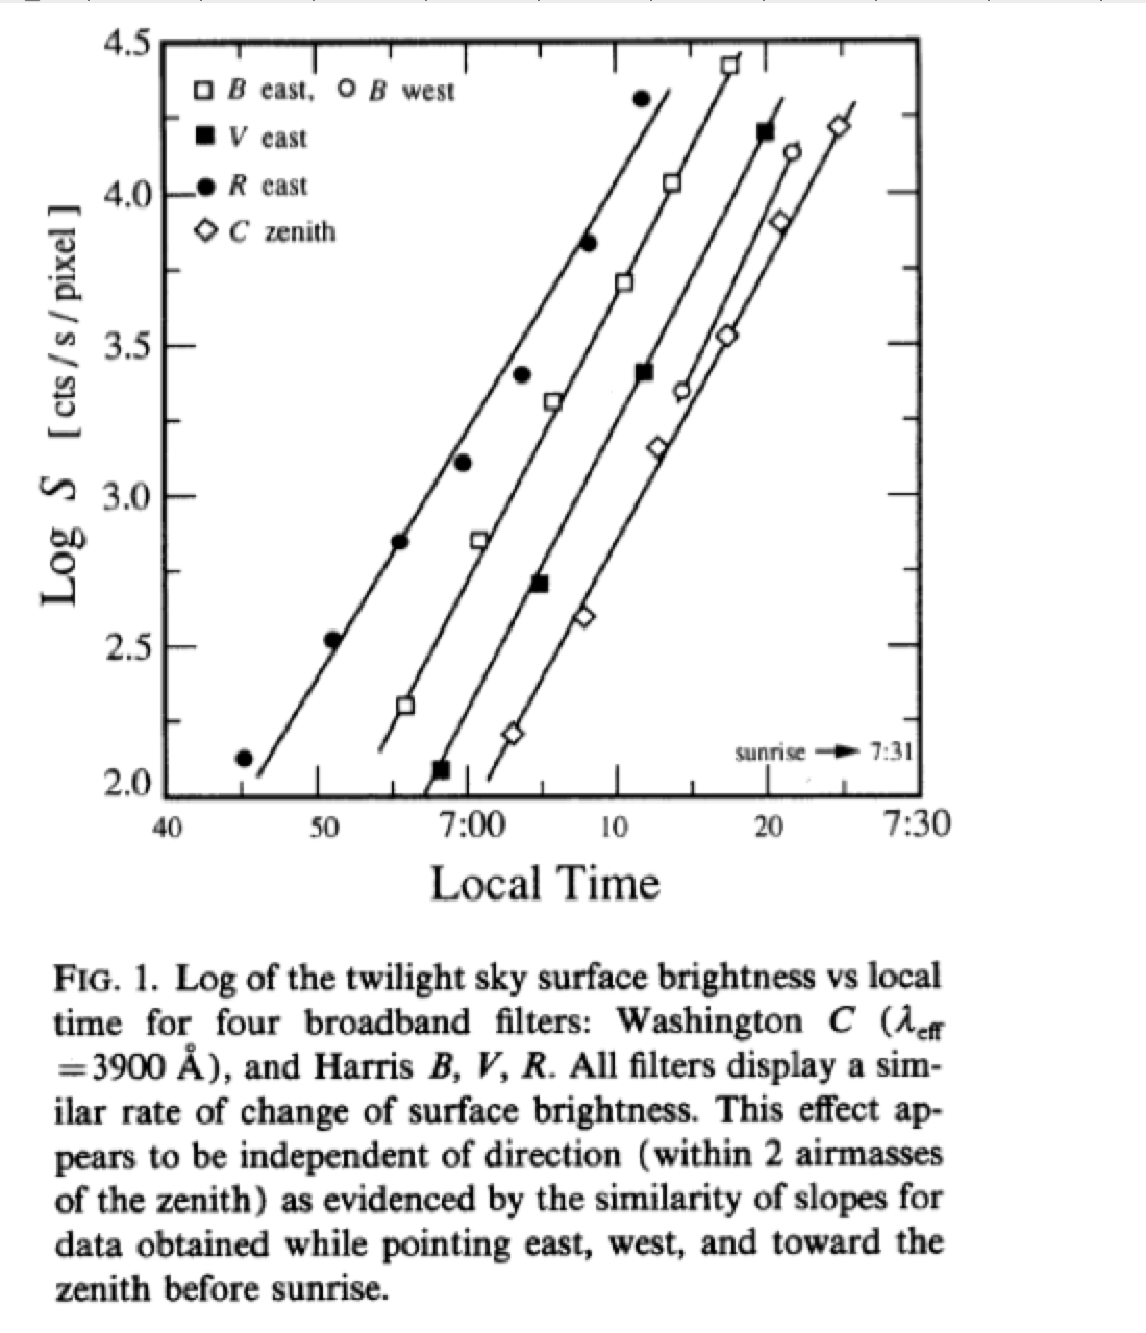
\includegraphics[width=6in]{figs/Stubbs_Fig1.pdf}
\caption{(reproduced from Tyson et al, 1993). This plot shows that the sky brightness changes by one magnitude in a 4.2 minute interval, essentially independent of passband.}
\label{default}
\end{center}
\end{figure}

Figure 2 illustrates the principles that underpin this proposal. LSST is a unique combination of hardware and software, that will deliver reliable catalogs of both the static and the dynamic sky. By pushing towards shorter integration times we can greatly expand the scientific reach of the system. 

The dynamic range in magnitudes that we can achieve for a given integration time depends on the sky background, the read noise, and the full well depth per pixel. We will adopt a typical value of 100Ke for the full well depth, but the arguments presented below are essentially independent of this value. The dynamic range in magnitudes is limited on the bright end by the point source whose PSF peak exceeds full well, and on the faint end by the 5$\sigma$ point source sensitivity, which depends on sky brightness per pixel. So we are squeezed between the two parameters of full well depth and sky background. 

\begin{figure}[htbp]
\begin{center}
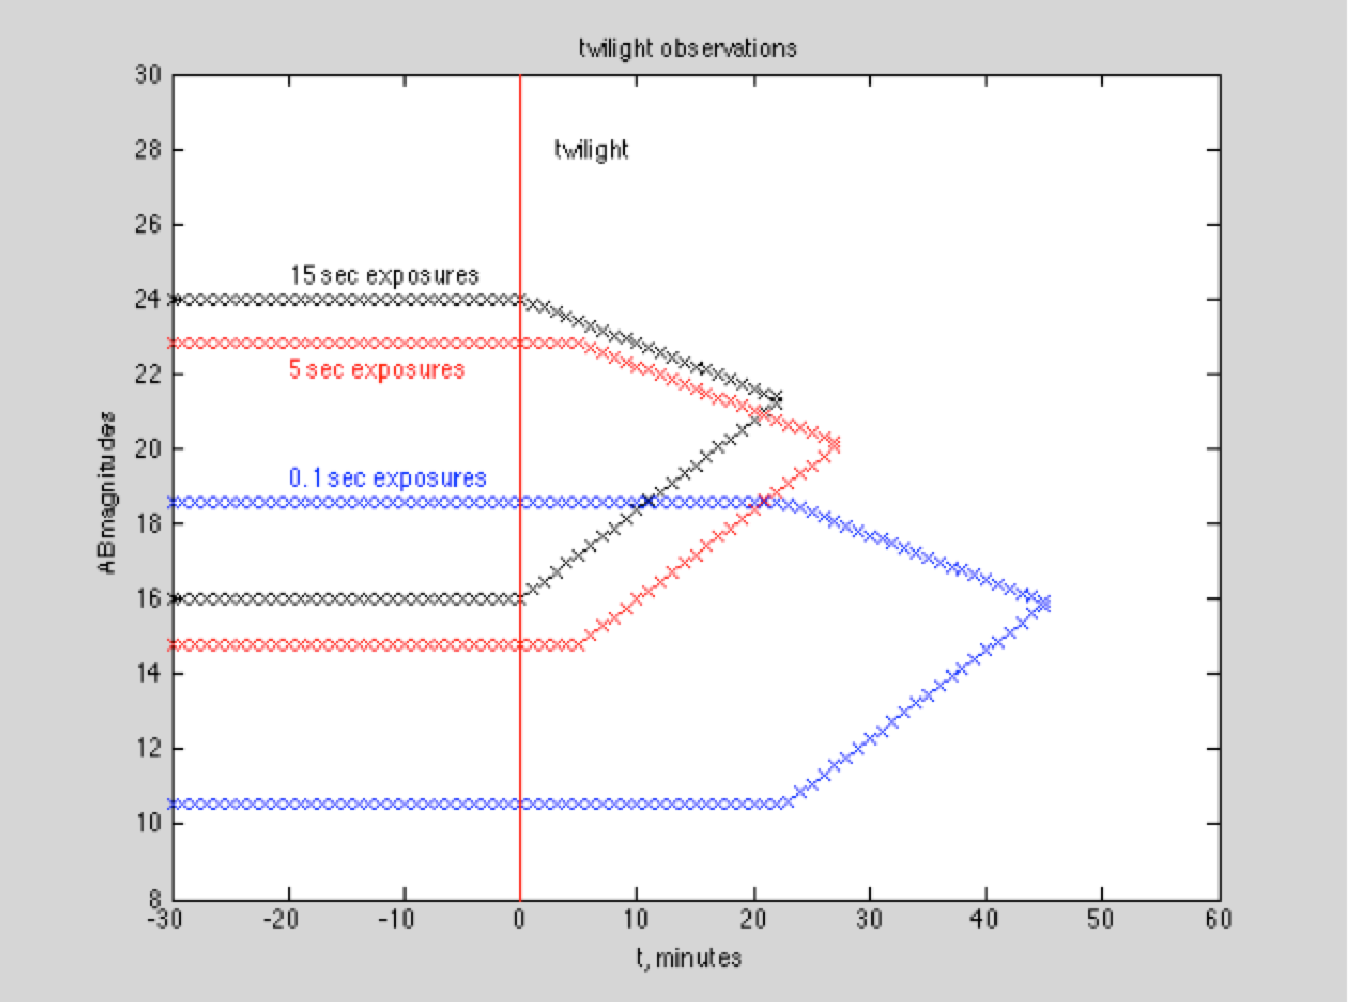
\includegraphics[width=6in]{figs/Stubbs_Fig2.pdf}
\caption{Twilight dynamic range. As we enter morning twilight time, the increasing sky brightness requires brighter sources for 5 sigma detection, and also limits unsaturated objects to increasingly fainter sources. Eventually the gap between these goes to zero. But operating at shorter exposure times allows us to push useful survey operations into brighter twilight time, and also to increase the dynamic range of the LSST survey products. The black lines correspond to 15 second integrations (nominally in the r band), the red lines to 5 second exposures, and the blue curves to 0.1 second exposures. The upper lines in each case represent the 5 sigma point source detection threshold while the lower line corresponds to the source brightness that produces saturation in the peak pixel of the PSF. Adding shorter exposure times increases our dynamic range in flux, and adds valuable observing time.}
\label{default}
\end{center}
\end{figure}

The 5 sigma limiting flux scales as the square root of the sky brightness, while the saturation flux decreases linearly as sky brightness increases. So the two curves in Figure 2 have slopes that differ by a factor of two. Operating during bright-sky time with short exposures adds about 20 minutes of observing per twilight, or 40 minutes per night. This is a non-trivial resource!

Figure 2 shows one reason why it is not advantageous to go below 0.1 second exposures- we would lose the overlap between a twilight survey and the standard LSST object catalog. 

Having set the stage for the opportunity to operate at shorter exposure times either during dark sky time, or during twilight, or both, we now describe some of the scientific motivations for doing so. 

\subsection{Science Drivers for Shorter Exposures}

\subsubsection{Discovery space at short time scales.} 

LSST is a time domain discovery machine. It is hard to anticipate the importance of being able to detect astronomical variability on short time scales. By extending the time domain sensitivity to phenomena with a characteristic time of less than 5 seconds, we will have added 1.5 orders of magnitude in time domain sensitivity. 

Taking short exposures does not necessarily imply a requirement on fast image cadence. Periodic variability can be readily detected and characterized with a succession of short images that do not satisfy the Nyquist criterion, as long as we know the time associated with each data point to adequate accuracy. But it does seem appropriate to investigate the maximum possible rapid-fire imaging rate for LSST, presumably limited by either data transfer bottlenecks or by thermal issues within the camera. 

\subsubsection{Distances to Nearby SN Ia- an essential ingredient in using supernovae to probe dark energy.}

The determination of the equation of state parameter of the Dark Energy using type Ia supernovae entails measuring the redshift dependence of the luminosity distances to objects over a range of redshifts. The low end of this redshift range is limited by peculiar velocities to considering supernovae at redshifts z$>$0.01. At this distance (distance modulus of 
$\mu$ =33) the peak brightness of a type Ia supernova is r=15 and exceeds the expected LSST point source saturation limit. 

Moreover, the rate on the sky of these bright nearby supernovae is so low that in the standard cadence we don�t expect to obtain well-sampled multiband light curves for them. But we will discover many of them on the rise. Using twilight time with short exposures to obtain appropriate temporal and passband coverage will allow us to extend the LSST SN Hubble diagram across the entire redshift range of 0.01 to 1. 

It is vitally important that we obtain these nearby-SN light curves on the same photometric system, reduced with the same data reduction pipeline, as the distant sample. This means we really must use the LSST instrument and software in order to avoid systematic errors arising from differences in photometric systems or algorithmic issues. 

We stress that this twilight SN followup campaign can be accomplished without impacting the main survey, during the roughly 20 minutes per night of twilight that would otherwise unusable at the default exposure time. We would use the brighter twilight time to obtain pointed observations on nearby supernovae, motivated by the importance of photometric uniformity described above. 

\subsubsection{A Bright Star Survey for Galactic Science.}

We could also use the added twilight time to conduct a bright star survey, and the precise astrometry and photometry from LSST can then be used in conjunction with archived data ranging from 11th to 27th AB magnitudes. This short-exposure domain would extend the LSST dynamic range in fluxes by two orders of magnitude, towards the bright end. Moreover, obtaining precise positions, fluxes and variability at these brighter magnitudes would greatly increase the overlap with the historical archive of astronomical information, including from digitized plate data. We would be able to obtain astrometric and color information to high precision, as well time series for variability studies. 

An example of an application to Milky Way structure studies comes from RR Lyrae variable stars. With a saturation magnitude of around 16th in the standard LSST survey, RR Lyrae closer than 20 kpc will be saturated in the standard LSST images. So we will lose nearly all Galactic RR Lyrae. Extending the survey�s bright limit to 11th magnitude will allow us to collect light curves for RR Lyrae beyond $\sim$ 100 parsecs, collecting essentially all Southern hemisphere Galactic RR Lyrae.

Another application for stellar population studies is measuring the fraction of binary stars as a function of stellar type, metallicity, age and environment. By conducting a variability survey in the 11-18 magnitude range we can capitalize on temperature and metallicity data already in hand for many of these objects. 

Another application of a bright star survey would be to search for planetary transits in the magnitude range appropriate for radial velocity followup observations using 30 meter class telescopes. For high dispersion spectrographs at the 4m aperture class, most targets are currently around 8th magnitude, so we should expect 30m telescopes to attain similar radial velocity precisions for sources of magnitude  8 + 5log(30/4) = 12. By going to shorter exposures we obtain almost an hour�s additional observing time per night when these sources don�t saturate, whereas they are far beyond saturation in the default 15 second LSST survey images. 

A typical (r$-$K) color between SDSS and 2MASS is r$-$K=3. The 2MASS catalog is complete down to K$\sim$14 which corresponds to r$\sim$17. So most 2MASS stars will be saturated in the standard LSST 15 second observations. A bright star survey will allow a multiband match to the 2MASS data, as well as an astrometric comparison between the two catalogs. 

Finally, the apparent magnitude of solar system objects depends on their distance from us and from the sun, as well as illumination and observation geometry. Extending the bright limit will allow us to track asteroid positions as they approach opposition.  

\subsection{Counterarguments}

\subsubsection{What About Scintillation Effects?}

Short exposure times suffer from scintillation effects. An estimate for uncertainty due to scintillation is provided by 
\url{http://astro.corlan.net/gcx/scint.txt}. For a 0.1 second integration we expect a fractional flux uncertainty of  0.15 at 2 airmasses and 0.043 at 1 airmass, for a 10 cm aperture. Scaling this up to the 8.5m aperture of LSST by a factor D$^{2/3}$ predicts fractional flux variations of below one percent, even at two airmasses, for a 0.1 second exposure. So scintillation should not impact our ability to make precision measurements of flux and position.  

\subsubsection{What about just doing this with smaller telescopes?}

A possible counter-argument to the proposal of allowing for shorter exposure times is that much of this can be done with smaller telescopes. But it�s important to bear in mind that LSST is a system, and the data reduction and dissemination tools are as important as the hardware. We intend to deliver accessible, high-quality, well-calibrated photometry on a common photometric system and correspondingly good positions. If we do so from a co-added point source depth of 27th to the short-exposure bright limit of 11th magnitude we will span over six decades in flux on a well-calibrated flux scale. We would also have the ability to study astrophysical variability on time scales from 0.1 second to 10 years, which is nine decades in the time domain. This combination of temporal and flux dynamic range would be a truly remarkable  achievement, and would yield science benefits far beyond the illustrative examples provided above. Much of this discovery space is enabled by going to shorter exposures. 
 
\subsection{Proposed Implementation and Impacts}

The implementation of this would simply entail taking short-exposure images during twilight time that would otherwise go unused. The data rate would go up, and the number of shutter cycles per night would also increase. 
%
%\section{References}
%
%Tyson and Gal, An Exposure Guide for Taking Twilight Flats with Large Format CCDs, AJ {\bf 105}, 1026 (1003). 




% --------------------------------------------------------------------

\navigationbar
